% begin module second-derivative-concavity
\begin{frame}
\begin{columns}[c]
\column{.5\textwidth}
\ 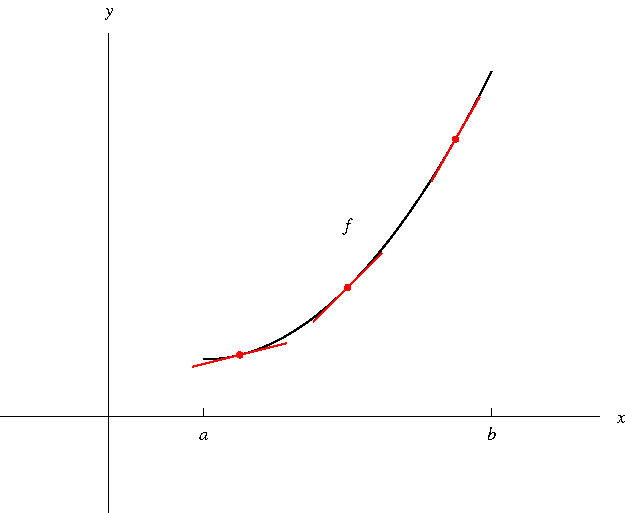
\includegraphics[height=3.5cm]{curve-sketching/pictures/04-03-concaveupe.pdf}%
\column{.5\textwidth}
\ 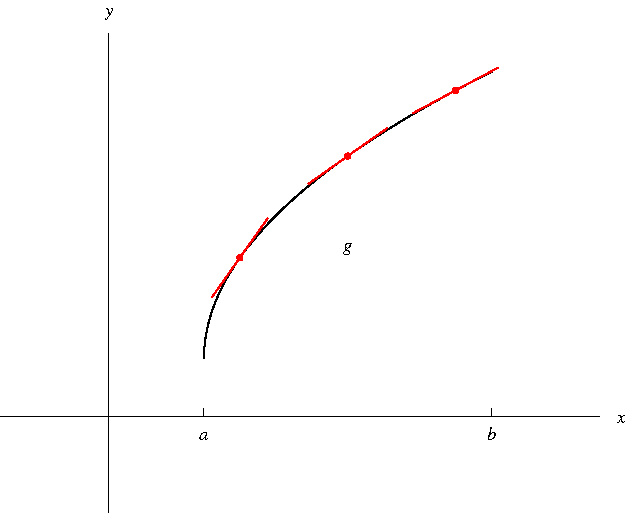
\includegraphics[height=3.5cm]{curve-sketching/pictures/04-03-concavedowne.pdf}%
\end{columns}
\begin{itemize}
\item  In the graph of $f$ the slopes of the tangent lines increase as we move from left to right.
\item<2->  This means $f'$ is an increasing function.
\item<3->  This means $f''$ is positive on $(a,b)$.
\item<4->  Similarly $g''$ is negative on $(a,b)$.
\end{itemize}
\uncover<5->{%
Concavity Test
\begin{enumerate}
\item  If $f''(x) > 0$ for all $x$ in $I$, then the graph of $f$ is concave up on $I$.
\item  If $f''(x) < 0$ for all $x$ in $I$, then the graph of $f$ is concave down on $I$.
\end{enumerate}
}%
\end{frame}
% end module second-derivative-concavity
